%-------------------------------------------------------------------------------
% architecture
%-------------------------------------------------------------------------------
%
% \file        architecture.tex
% \library     Documents
% \author      Chris Ahlstrom
% \date        2024-03-07
% \update      2024-04-06
% \version     $Revision$
% \license     $XPC_GPL_LICENSE$
%
%     Provides a description of the classes and modules of this library.
%
%-------------------------------------------------------------------------------

\section{Potext Architecture}
\label{sec:potext_architecture}

   This section provides a walk-through of the architecture
   of the \textsl{Potext} library.
   Much of the architecture is similar to \textsl{Tinygettext}
   (\cite{tinygettext}), but
   there are some important changes and additions.
   Some notes about the classes and documentation:

   \begin{itemize}
      \item All classes and free functions are wrapped in the
         \texttt{po} namespace.
      \item The macro \texttt{\_()} that normally wraps \textsl{GNU} function
         \texttt{gettext()} here wraps the \textsl{Potext} function
         \texttt{po::gettext()}.
      \item The related "gettext" functions are redefined in terms of
         \textsl{Potext} functions.
      \item In the diagrams, for the function parameters, we use
         "std::string", rather than "const std::string \&" for brevity in the
         diagrams.
      \item Not every attribute or function is described. Some groups of
         items include \texttt{\_xxxx\_} to represent a number of similar
         functions.
      \item The copy constructors, principal assignment operators, and
         destructors are not described. See the header files to see
         if they are \texttt{default}, \texttt{delete}, or defined.
   \end{itemize}

   First, the big picture.

\begin{figure}[H]
   \centering 
   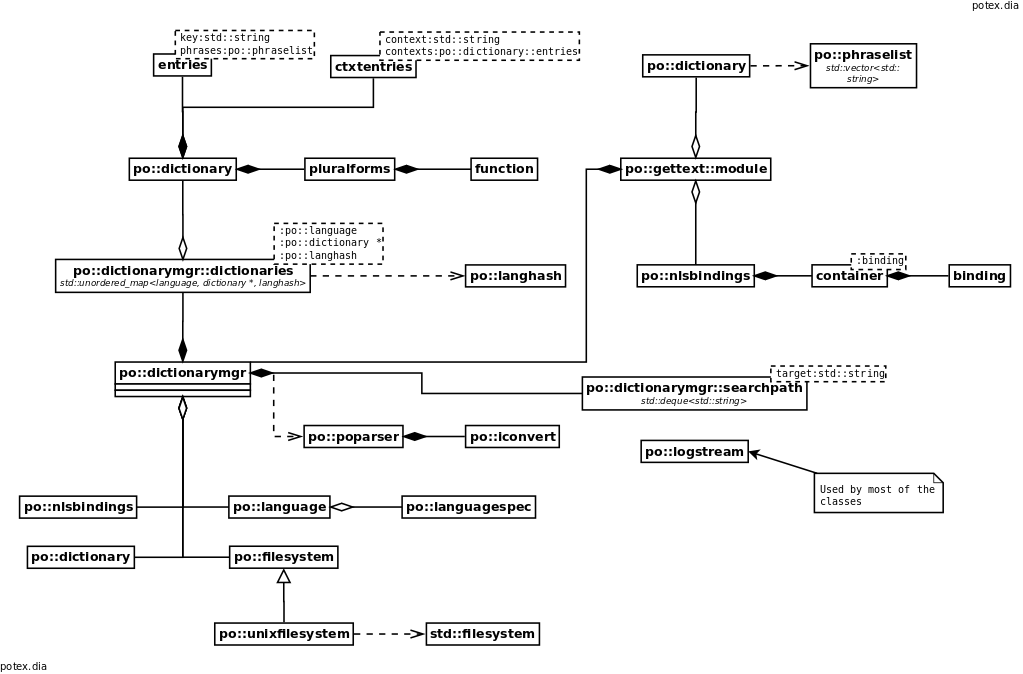
\includegraphics[scale=0.65]{potext.png}
   \caption{Potext "Big Picture" Architecture}
   \label{fig:potext}
\end{figure}

   The most important part of \textsl{Potext} is the
   \texttt{dictionary} class.
   It is filled by the \texttt{po::poparser::parse()} function,
   which takes a \texttt{.po} file and fills a dictionary object
   with a set of message strings and their translations.
   It also includes plural forms from the \texttt{.po} file to
   translate plural messages using "plural" functions.
   Each dictionary includes the message entries and context entries.
   For a description of the \texttt{.po} file, see
   the \textsl{GNU Gettext} manual (\cite{gettextman}).

   The \texttt{dictionarymgr} class handles one or more dictionaries.
   It has been augmented to hold a new \texttt{nlsbindings} class toion
   provided support for \texttt{bindtextdomain} and \texttt{textdomain},
   which are \textsl{not} provided by \textsl{Tinygettext}.

   The \texttt{dictionarymgr}'s additional member functions are used
   to implement the free functions in the \texttt{gettext} module, such
   as \texttt{gettext()} and \texttt{dgettext()},
   etc.
   The \texttt{gettext} module is an addition to \textsl{Potext} to
   make it easy to switch from \textsl{Gettext} to \textsl{Potext}.

   The \texttt{language} class supports the various parts of
   a domain name: language, country, modifier, long name, and the
   long name localized.

   Parsing \texttt{.po} files is facilitated by the various file-system
   classes. Each \texttt{.po} file results in the creation of a dictionary.

   The \texttt{poparser} class supports reading and parsing a
   \texttt{.po} file to create a \texttt{dictionary}.
   It inherits some common code from the
   \texttt{pomoparserbase} class.

   The \texttt{moparser} class supports reading and parsing a
   \texttt{.mo} file to create a \texttt{dictionary}.
   It also inherits some common code from the
   \texttt{pomoparserbase} class.

   The \texttt{iconvert} class supports converting the translations
   to another codeset (besides \texttt{UTF-8}) when creating the
   dictionaries.

   The \texttt{logstream} class supports internal error logging,
   but can also be used by an application.

   These classes are discussed in more detail in the following sections.

\subsection{Logstream Class}
\label{subsec:potext_logstream_class}

   The \texttt{po::logstream} class is a reimplementation of the
   \texttt{tinygettext::Log} class.

\begin{figure}[H]
   \centering 
   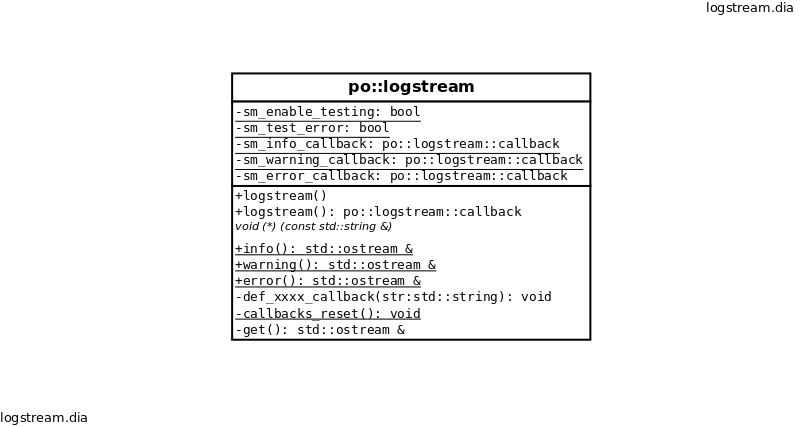
\includegraphics[scale=0.80]{logstream.png}
   \caption{Log Stream (po::logstream)}
   \label{fig:potext_logstream}
\end{figure}

   The \texttt{po::logstream} class provides \texttt{std::ostream}
   objects for emitting errors, warnings, and information messages.
   It also provides the ability to set a callback function to
   change how the messages are emitted.
   It is used internally for writing status to the console.
   It can also be used by an application, but ...

   ... An interesting issue that we have not yet figured out is
   illustrated by the test application \texttt{hellopotext}.
   When run, all of the messages written to \texttt{std::cout}
   appear first, including the final message "SUCCESS".
   Then all of the messages logged during setup and translation in the
   \textsl{Potext} library appear when \texttt{hellopotext}
   is \textsl{exiting}.

\subsection{Dictionary Manager Class}
\label{subsec:potext_dictionarymgr_class}

   The \texttt{po::dictionarymgr} class is a reimplementation of the
   \texttt{tinygettext::dictionary\_manager} class.
   It contains an \texttt{std::unordered\_map} of
   shared pointers to \texttt{dictionary} objects, keyed by
   \texttt{language} objects which are searched using
   \texttt{operator ()} hash function in a \texttt{po::langhash}
   structure.

   Currently, \textsl{Potext} does not do anything special with the
   \texttt{searchpath} deque.

% TODO
% Add the new get_dictionary() function to the diagram.
% TODO

\begin{figure}[H]
   \centering 
   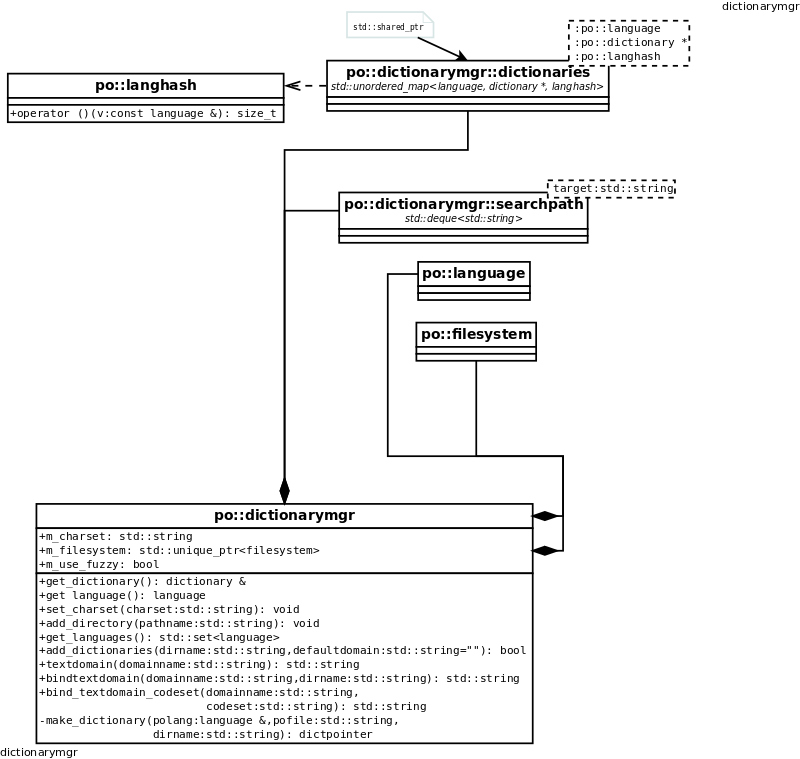
\includegraphics[scale=0.80]{dictionarymgr.png}
   \caption{Dictionary Manager (po::dictionarymgr)}
   \label{fig:potext_dictionarymgr}
\end{figure}

   In \textsl{Tinygettext}, the \texttt{dictionary\_manager} class 
   coordinated multiple locale directories and the selection of
   a particular \texttt{dictionary} for a translation.

   \textsl{Potext}'s \texttt{dictionarymgr}
   currently handles only one directory, but it
   adds support for domain-binding and for actually using translation
   functions that accept a domain parameter.
   The new functions are described next.

   \begin{itemize}
      \item \texttt{get\_bindings()}. This function returns an
         \texttt{nlsbindings} class reference that contains a list of domain
         names with the names of the directory and the character-set
         for each domain.
         The \texttt{nlsbindings} class provides the set-binding functions
         needed by the following new functions.
      \item \texttt{add\_dictionaries()}.
         This function scans a directory for \texttt{.po} files
         and creates a \texttt{dictionary} for each one.
      \item \texttt{make\_dictionary()}.
         This helper function opens a file using the \texttt{std::filesystem}
         class function \texttt{open\_file}.
         It then creates an \texttt{std::shared\_ptr} for a new
         \texttt{dictionary} and calls the static function
         \texttt{po::poparser::parse\_po\_file()}.
         Then it calls the member function
         \linebreak \texttt{po::nlsbindings::set\_binding\_values()}
         to create a corresponding binding object.
      \item \texttt{textdomain()}.
         This function sets the current domain to the given domain name.
         It is used in the \texttt{gettext} module to
         implement the \texttt{textdomain()} function.
      \item \texttt{bindtextdomain()}.
         This function associates a domain name with a locale directory
         in which to find the \texttt{.po} file.
         It is used in the \texttt{gettext} module to
         implement the \texttt{bindtextdomain()} function.
      \item \texttt{bind\_textdomain\_codeset()}.
         This function associates a domain name with a character-set to
         use in converting messages.
         It is used in the \texttt{gettext} module to
         implement the \texttt{bind\_textdomain\_codeset()} function.
      \item \texttt{get\_dictionary()}.
   \end{itemize}

\subsection{Pomoparserbase Class}
\label{subsec:potext_pomoparserbase_class}

   As of version 0.2, some common functionality has been moved into
   this base class.

\begin{figure}[H]
   \centering 
   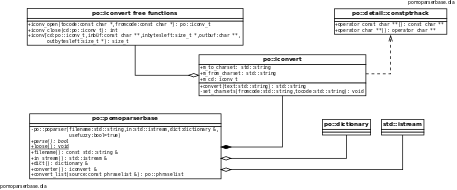
\includegraphics[scale=0.65]{pomoparserbase.png}
   \caption{PO/MO Parser Base (po::pomoparserbase)}
   \label{fig:potext_pomoparserbase}
\end{figure}

   For version 0.2, we have moved the file-reading support, dictionary class,
   and \texttt{iconvert} class
   into a base class common to the \texttt{moparser} and
   \texttt{poparser} classes.

   Other than that commonality, the two parser class are somewhat different in
   how they parse, since the \texttt{.po} file is text, and
   the \texttt{.mo} file is binary.

\subsection{Poparser Class}
\label{subsec:potext_poparser_class}

   The \texttt{po::poparser} class is a serious reimplementation of the
   \texttt{tinygettext::POParser} class.

\begin{figure}[H]
   \centering 
   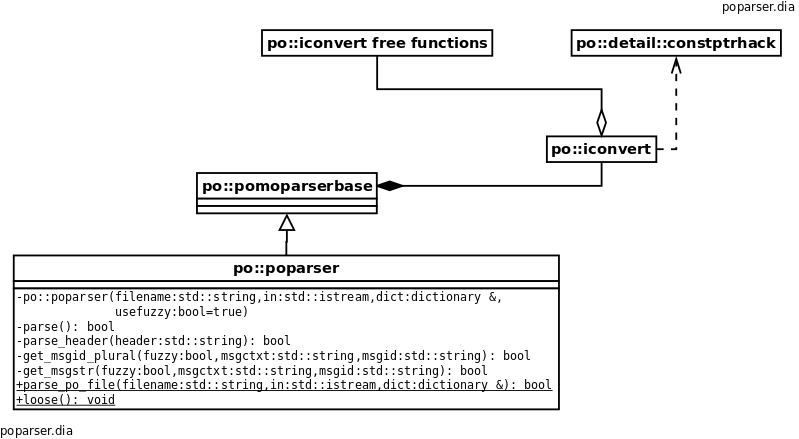
\includegraphics[scale=0.4]{poparser.png}
   \caption{PO Parser (po::poparser)}
   \label{fig:potext_poparser}
\end{figure}

   The \texttt{poparser} "connects" a \texttt{.po} file, an input stream,
   and a \texttt{dictionary} object in order to populate the dictionary with
   plural forms, set the character-set, and use it (if needed) to convert the
   translated message string to the character-set,
   The static function \texttt{po::poparser::parse\_po\_file()} is called to
   create a temporary \texttt{poparser} and use it to
   read a file and fill in an empty \texttt{dictionary}.

   The \texttt{po::poparser::get\_string\_line()} function handles the
   main task of parsing a line from the \texttt{.po} file and deciding
   what to do with it.

   The \texttt{po::poparser::get\_msgstr} function adds a message (which might
   be converted to a specified character-set) to the dictionary.

   The \texttt{po::poparser::get\_msgid\_plural()} adds a plural form
   (see \sectionref{subsec:potext_pluralforms_class})
   or a contextual translation to the dictionary.

%  We need to follow up and make sure that each translation in the list of
%  translations is converted to a specified character-set if applicable.

   The \texttt{po::poparser} class uses the \texttt{po::iconvert} class
   to convert the string translation to the desired character-set.
   The \texttt{po::iconvert} class is a reimplementation of the
   \texttt{tinygettext::IConv} class.
   Note that it defines the \texttt{po::iconv\_t} type.

\subsection{Moparser Class}
\label{subsec:potext_moparser_class}

   The \texttt{po::moparser} class is based on \texttt{pomoparserbase},
   and adds the ability to parse \texttt{.mo} files.
   \texttt{tinygettext::POParser} class.

\begin{figure}[H]
   \centering 
   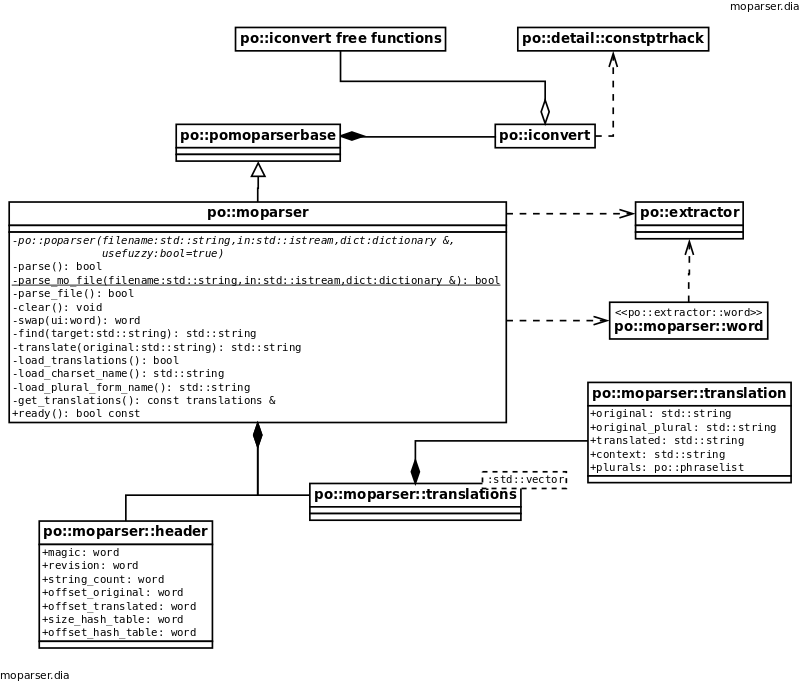
\includegraphics[scale=0.65]{moparser.png}
   \caption{MO Parser (po::moparser)}
   \label{fig:potext_moparser}
\end{figure}

   The \texttt{moparser} "connects" a \texttt{.mo} file, an input stream,
   and a \texttt{dictionary} object in order to populate the dictionary with
   plural forms, set the character-set, and use it (if needed) to convert the
   translated message string to the character-set,
   The static function \texttt{po::moparser::parse\_mo\_file()} is called to
   create a temporary \texttt{moparser} and use it to
   read a file and fill in an empty \texttt{dictionary}.

   The format of the \texttt{.mo} file is described in the \texttt{moparser}
   module's top banner. The format is dissected and described further in these
   files:

   \begin{verbatim}
      library/tests/mo/es/newt.hex
      library/tests/mo/de/helloworld.hex
   \end{verbatim}

   Note the \texttt{moparser::header} structure, which provides
   the layout of the first few words in the \texttt{.mo} file.
   Each \texttt{translation} structure holds the "original" message ID,
   the "original plural" message ID, the context (if specified),
   the translated singular string, and a list of plural forms (if specified).

   The \texttt{moparser} class gets the character-set name and the
   plural-forms description by searching for the key strings to find them.
   It then searches for original singular strings, original
   plural strings, context strings, and the list of plural translations.
   These items are stored in a vector of translations, which is later
   used to populate a \texttt{dictionary}.

   The process of the binary data is facilitated by the \texttt{extractor}
   class discussed in the next section.

\subsection{Extractor Class}
\label{subsec:potext_extractor_class}

   This new class is used internally in the parsing of \texttt{.mo}
   files. It encapsulates some tricky binary data extraction
   so that the \texttt{moparser} class is less complex than otherwise.
   The binary data is represented by a string, which is loaded by the
   constructor.

\begin{figure}[H]
   \centering 
   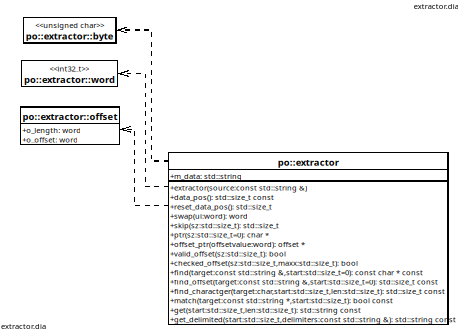
\includegraphics[scale=0.4]{extractor.png}
   \caption{Binary Data Extractor (po::extractor)}
   \label{fig:potext_extractor}
\end{figure}

   For the most part, the data in the string is accessed by position and
   length. Offsets and pointers for string or character targets can be
   found using a starting offset, a length, and perhaps a character delimiter
   such as a newline, null byte, and the EOT (ASCII 4) character.

   Note the data types of \texttt{byte} and \texttt{word}, here hidden in the
   extractor class.

   Also included is the \texttt{offset} structure, which is the pair of data
   items the \texttt{.mo} format uses.

\subsection{Dictionary Class}
\label{subsec:potext_dictionary_class}

   The \texttt{po::dictionary} class is a reimplementation of the
   \texttt{tinygettext::Dictionary} class.

\begin{figure}[H]
   \centering 
   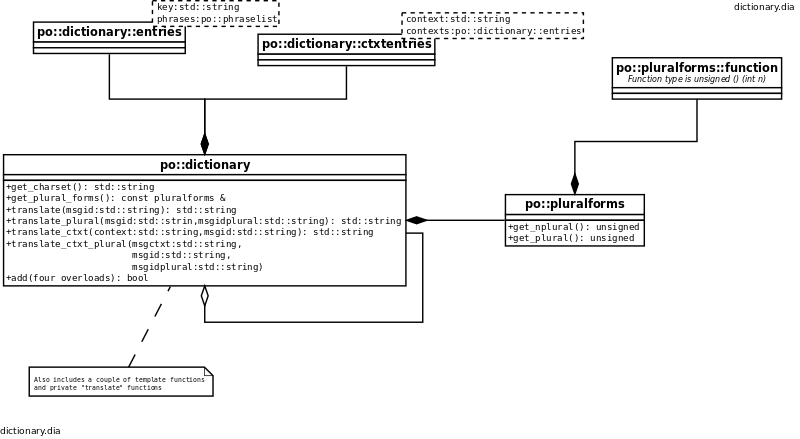
\includegraphics[scale=0.80]{dictionary.png}
   \caption{Dictionary (po::dictionary)}
   \label{fig:potext_dictionary}
\end{figure}

   The \texttt{dictionary} class holds a set of conversions of strings to a
   list of possible conversions, and another set of lists to support various
   message contexts.

   The dictionary contains \texttt{entries}, an \texttt{std::unordered\_map}
   of phrases keyed by a message ID string as used in \textsl{GNU}
   \texttt{gettext()}.
   A \texttt{phraselist} is simply an \texttt{std::vector<std::string>}.

   The dictionary also contains \texttt{ctxtentries},
   an \texttt{std::unordered\_map} of \texttt{entries} keyed by a
   context string.

   The dictionary also contains a \texttt{pluralforms} object that can be used
   to look up the proper plural translation.
   These functions provide the desired lookups:

   \begin{itemize}
      \item \texttt{translate()}. 
      \item \texttt{translate\_plural()}. 
      \item \texttt{translate\_ctxt()}. 
      \item \texttt{translate\_ctxt\_plural()}. 
   \end{itemize}

   Note that there are no functions that use the name of a domain as
   a parameter.
   Instead, the domain-using functions in the \texttt{gettext} module
   look up the dictionary associated with the desired domain, 
   and use the appropriate translate function.

   The \texttt{pluralforms} class deserves its own small section.

\subsection{Pluralforms Class}
\label{subsec:potext_pluralforms_class}

   The \texttt{po::pluralforms} class is a reimplementation of the
   \texttt{tinygettext::PluralForms} class.
   Each \texttt{.po} file contains a line describing how the translation of
   plurals is to be handled for each language:

   \begin{verbatim}
      Plural-Forms: nplurals=2; plural=n != 1;
   \end{verbatim}
   
   The \texttt{pluralforms} class provides a static function for each
   possible plural form (and there are quite a number of them).
   These functions are inserted into an \texttt{std::unordered\_map}
   which is keyed by strings like the one shown above.
   Some of these strings are extremely long.
   \textsl{(We could shorten the keys by ignoring the redundant part
   of the plural-forms string.)}

   The \texttt{po::pluralforms::from\_string()} function strips the
   spaces from a string parameter and does a fast lookup to return the
   appropriate \texttt{pluralforms} object.

\subsection{Language Class}
\label{subsec:potext_language_class}

   The \texttt{po::language} class is a reimplementation of the
   \texttt{tinygettext::Language} class.

   The \texttt{po::languagespec} structure is a reimplementation of the
   \texttt{tinygettext::LanguageSpec} structure.
   This structure now uses \texttt{std::string} instead of character pointers.

\begin{figure}[H]
   \centering 
   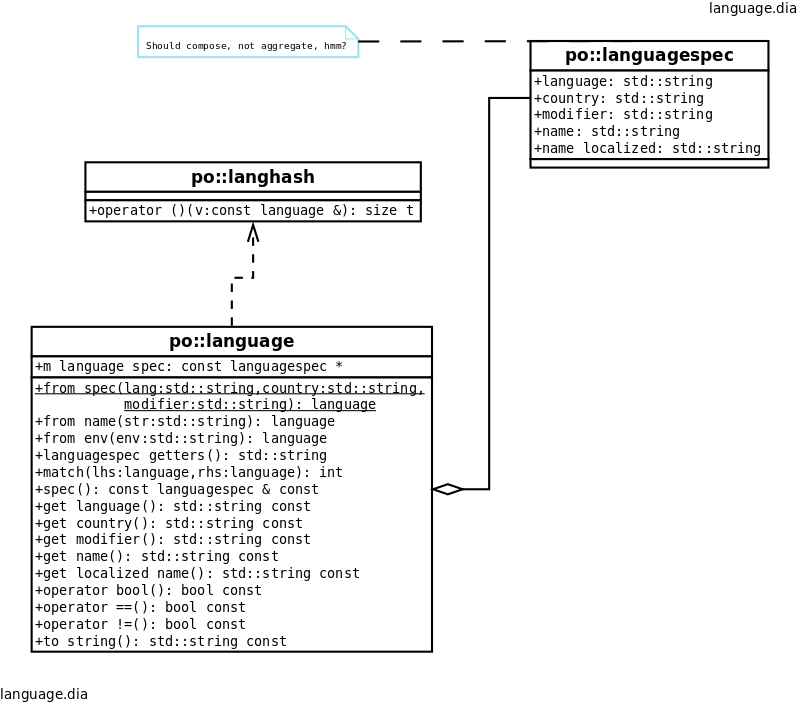
\includegraphics[scale=0.75]{language.png}
   \caption{Language (po::language)}
   \label{fig:potext_language}
\end{figure}

   The \texttt{language} class is a wrapper for a
   \texttt{languagespec} structure.
   As shown in the figure, it provides functions to get and set the
   components of a language specification, to make comparisons, and
   converted the specification to a string.

   The \texttt{dictionarymgr} uses the
   \texttt{language} as a key to look up the desired dictionary, and
   if not found, to make a new dictionary and add it to the dictionary
   container.

% TODO
   We still need to understand a little more about this class and its usage.
% TODO

\subsection{NLS Bindings Class}
\label{subsec:potext_nlsbindings_class}

   The \texttt{nlsbindings} class is an addition for the \textsl{Potext}
   library to support adding text-domain functions akin to those in
   \textsl{GNU Gettext}, but wrapped in the \texttt{po} namespace.

\begin{figure}[H]
   \centering 
   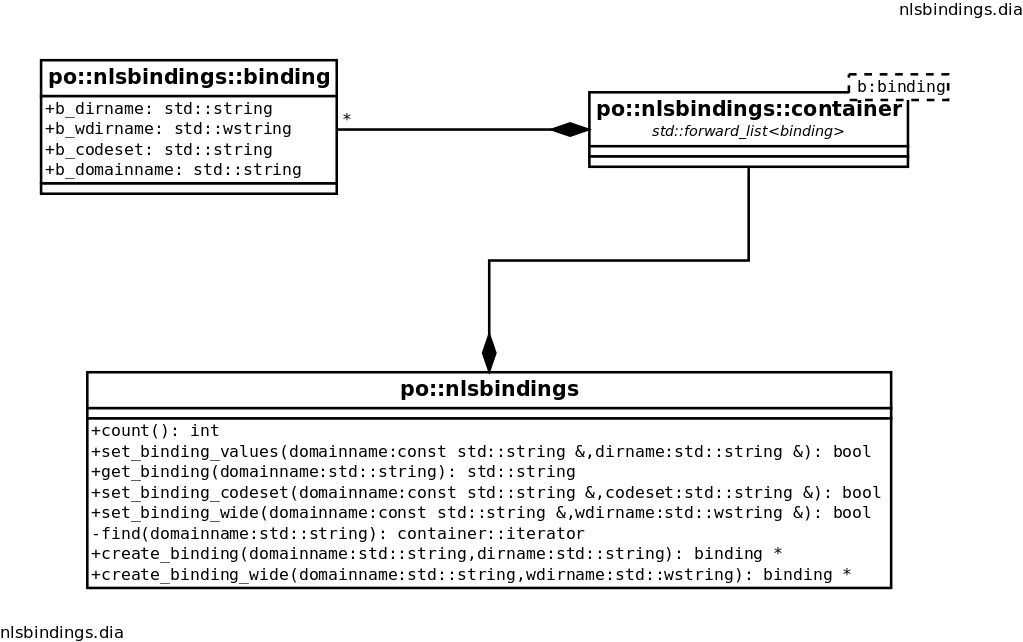
\includegraphics[scale=0.9]{nlsbindings.png}
   \caption{NLS Bindings (po::nlsbindings)}
   \label{fig:nlsbindings}
\end{figure}

   It provides some simplified implementations of
   \textsl{GNU Gettext} functions that lack such niceties as
   locking and checking for SUID root applications.
   These can be added later as the need becomes apparent.
   For details, see the code in the 
   \textsl{GNU Gettext} project in it's
   \texttt{gettext-runtime/intl} directory.

\subsection{Gettext Module}
\label{subsec:potext_gettext_module}

   The \textsl{Potext} \texttt{gettext} module is discussed in the next
   section.
   (See \sectionref{subsec:gettext_module}.)

%-------------------------------------------------------------------------------
% vim: ts=3 sw=3 et ft=tex
%-------------------------------------------------------------------------------
